%!TEX encoding = UTF-8 Unicode
%!TEX root = ../compendium.tex

\chapter{Dokumentation}\label{appendix:doc}

Dokumentation hjälper andra att använda din kod, men underlättar även för dig själv när du vid ett senare tillfälle ska erinra dig hur den fungerar och hur du ska använda och bygga vidare på din kod. Modern systemutveckling baseras ofta på öppen källkod och färdiga api \Eng{application programming interface}, där kvaliteten på dokumentationen är avgörande för hur lätt det är att komma igång med att använda koden.

Nedan listas exempel på olika typer av  dokumentation\footnote{\href{https://en.wikipedia.org/wiki/Software_documentation}{en.wikipedia.org/wiki/Software\_documentation}}:

\begin{itemize}
\item \textbf{Kravdokumentation} beskriver det övergripande målet med mjukvaran, samt funktionella krav och kvalitetskrav som uppfylls av systemet.
\item \textbf{Designdokumentation} beskriver arkitekturen, hur koden är organiserad i moduler, och den interna systemstrukturen t.ex. i form av klasser, objekt och deras relation.
\item \textbf{Slutanvändardokumentation} kan t.ex. vara manualer för användning av systemet och installationsanvisningar.
\item \textbf{Teknisk dokumentation} kan t.ex. vara api-dokumentation som beskriver vilka funktioner som ingår i ett programbibliotek. Sådan dokumentation genereras ofta med hjälp av ett \textbf{dokumentationsverktyg} (se avsnitt \ref{appendix:buildtool}).  Andra typer av teknisk dokumentation är instruktioner om hur man bygger koden med eventuellt tillhörande byggverktygskonfigurationsfiler; ofta beskrivs byggförfarandet steg för steg i en textfil med namnet \code{README}. (Läs mer om byggverktyg i appendix \ref{appendix:build}.) 
\end{itemize}

\noindent Det är en stor utmaning att hålla dokumentationen uppdaterad allteftersom koden utvecklas. Även om man får hjälp att generera en navigerbar sajt av ett dokumentationsverktyg, måste själva \textit{innehållet} i de manuellt författade dokumentationskommentarerna vara i överensstämmelse med den aktuella versionen av koden. Uppdateras koden, måste man alltså vara noga med att uppdatera dokumentationskommentarerna, annars uppstår stor förvirring. 

Detta problem är så pass allvarligt att man ska tänka sig noga för hur man kan formulera  dokumentationskommentarerna på ett framtidssäkert sätt, och hur omfattande de ska vara i förhållande till den framtida arbetsinsatsen med att hålla dem uppdaterade. Desto mer omfattande kommentarer desto mer jobb att hålla dem uppdaterade. 

Det är i praktiken svårt att uppnå en optimal balans mellan bra och många kommentarer som \textit{hjälper} användaren, och å andra sidan svårunderhållna och föråldrade kommentarer som \textit{stjälper} användare.


\section{Vad gör ett dokumentationsverktyg?}\label{appendix:buildtool}

Ett dokumentationsverktyg genererar teknisk dokumentation av koden baserat på speciella \textbf{dokumentationskommentarer} som skrivs i koden omedelbart före deklarationer av det som ska dokumenteras. Dessa dokumentationskommentarer skrivs enligt en speciell syntax som dokumentationsverktyget kan tolka.

Utdata från ett dokumentationsverktyg utgörs typiskt av en webbsajt med ändamålsenlig formatering och navigationslänkar, se figur \ref{fig:appendix:doctool}.

\begin{figure}[H]
\centering
\begin{tikzpicture}[node distance=1.8cm, scale=1.5]
\node (input) [startstop] {\bf\sffamily Källkod};
\node(inptext) [right of=input, text width=6cm, xshift=4.2cm]{med speciella dokumentationskommentarer före deklarationer};
\node (compile) [process, below of=input] {\bf\sffamily Dokumentationsverktyg};
%\node(explain) [right of=compile, text width=5cm, xshift=3.0cm]{Översätter från källkod till maskinkod};
\node (output) [startstop, below of=compile] {\bf\sffamily Dokumentation};
\node(outtext) [right of=output, text width=6cm, xshift=4.2cm]{t.ex. en webbsajt med dokumentation och navigationslänkar};
\draw [arrow] (input) -- (compile);
\draw [arrow] (compile) -- (output);
\end{tikzpicture}
    \caption{Ett dokumentationsverktyg läser koden och dokumentationskommentarer och genererar dokumentation, t.ex. i form av en webbsajt.}
    \label{fig:appendix:doctool}
\end{figure}



\section{scaladoc}
\newcommand{\scaladoc}{\texttt{scaladoc}}

Med Scala-installationen följer dokumentationsverktyget \scaladoc, som genererar en webbsajt med ändamålsenlig layout och specialfunktioner för att söka, filtrera och navigera i dokumentationen. 

Dokumentationen av stora bibliotek kan bli omfattande och det krävs träning i att använda dokumentationssajter för att få maximal nytta av dem. I efterföljande avsnitt beskrivs först hur du använder dokumentation som är genererad med \scaladoc. Därefter visas hur du själv kan generera dokumentation för din egen kod.


\subsection{Använda dokumentation från scaladoc}

Dokumentationen av Scalas standardbiliotek är genererad med \scaladoc~och att navigera i denna ger bra träning i hur man använder avancerad api-dokumentation. Du hittar dokumentationen för Scalas standardbibliotek här: \\
\url{http://scala-lang.org/api/current} 


När du surfar dit möts du av dokumentationen för \textit{root package}, som ger en översikt av olika paket i standardbiblioteket. I sökrutan uppe till vänster kan du skriva början på namnet på klasser, traits, eller objekt som du letar efter, så som visas i figure \ref{fig:scaladoc:root-package}.

\begin{figure}[H]
\centering
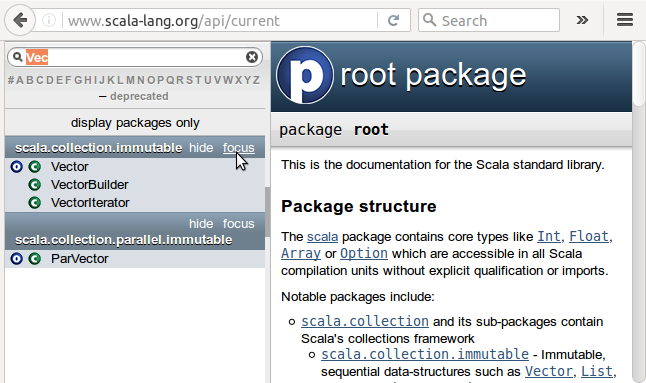
\includegraphics[width=0.8\textwidth]{../img/scaladoc/scaladoc-root}

     \caption{ \scaladoc.}
    \label{fig:scaladoc:root-package}
\end{figure}

Om du är speciellt intresserad av, t.ex., paketet \code{scala.collection.immutable}, kan du klicka \textbf{focus} för att begränsas visningen till att endast innehålla typerna i detta paket.

Om du söker efter typen där en viss metod är implementerad, men inte vet riktigt i vilken klass den finns, kan du klicka på bokstaven som metodnamnet börjar på i listan med bokstäver under den övre vänstra sökrutan. Då får du en lista med allt möjligt som börjar på F, så som visas i figur \ref{fig:scaladoc:find}. Sök i listan med din webbläsares sökfunktion (Ctrl+F) efter ''fill'', så hittar du alla typer som implementerar metoden \code{fill}. 

\begin{figure}[H]
\centering
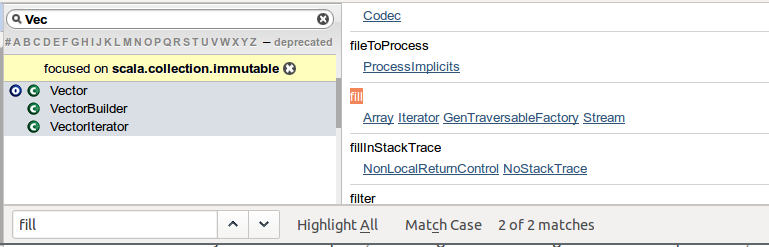
\includegraphics[width=1.0\textwidth]{../img/scaladoc/scaladoc-find-fill}

     \caption{ \scaladoc.}
    \label{fig:scaladoc:find}
\end{figure}

Om du klickar vidare, i detta exempel på länken till klassen Array, kan du sedan klicka på länken till källkoden i \texttt{array.scala} för att se implementationen på GitHub; sök på sidan med din webbläsares sökfunktion Ctrl+F efter ''def fill''.





Om du klickar på den typ du är intresserad av, t.ex. klassen Vector, får du upp en sida med en mängd information, inklusive alla metoder, även ärvda. Figur \ref{fig:scaladoc:vector} visar hur en sökning bland alla metoder i Vector initieras i sökrutan nere till höger, vilken kommer att visa metoder som börjar på ''rev'', här skrollas fönstret till metoden \code{reverse} längre ner på sidan.

Genom att klicka på det den gröna cirkeln med bokstaven C överst i dokumentationsfönstret, växlar du till vyn för kompanjonsobjektet där du hittar alla fabriksmetoder för Vector, även ärvda, t.ex. \code{fill} som du kan söka efter i sökrutan. 



\begin{figure}[H]
\centering
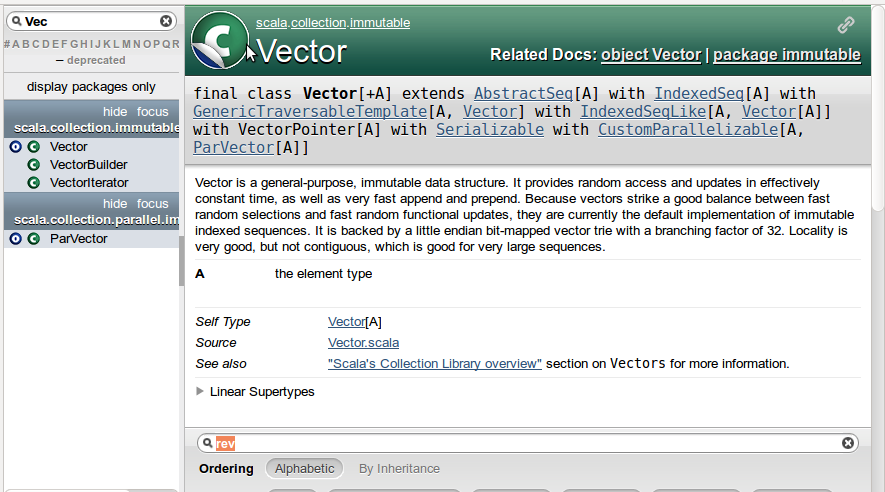
\includegraphics[width=1.0\textwidth]{../img/scaladoc/scaladoc-vec}

     \caption{ \scaladoc.}
    \label{fig:scaladoc:vector}
\end{figure}


\subsection{Skriva dokumentationskommentarer för scaladoc}


Verktyget \scaladoc~läser kommentarer som börjar med \verb|/**| och slutar med \verb|*/| och associeras till efterföljande deklaration. Notera de dubbla asteriskerna. Alla rader som följer efter \verb|/**| ska, enligt konventionen för Scalas dokumentationskommentarer, börja med en asterisk \code|*| med indrag med flera blanksteg så att den hamnar under \textit{andra} asterisken i öppningskommentaren, som nedan:
\begin{Code}
/** Först kommer en sammanfattning på en enda rad. 
  * 
  * Sedan kommer eventuellt en mer detaljerad beskrivning, 
  * som kan vara flera rader lång.
  */
\end{Code}
Dokumentationskommentaren slutar med \code|*/| rakt under asterisk-kolumnen.

I figur \ref{fig:scaladoc:mio} på sidan \pageref{fig:scaladoc:mio} visas exempel på dokumentationskommentarer. Annoteringen \verb|@param| i början på en rad ger en speciell kommentar angående parametrar. Annoteringen \verb|@return| i början av en rad ger en speciell kommentar angående vad som returneras vid metodanrop.


\subsection{Generera dokumentation med scaladoc}


Du genererar en dokumentationssajt med terminalkommandot \scaladoc~följt av en eller flera källkodsfiler. Med optionen \code{-d} anger du i vilket bibliotek sajten ska sparas. Du visar sajten genom att öppna filen \code{index.html} i en webbläsare. Nedan visas hur dokumentationen genereras för källkodsfilen i figur \ref{fig:scaladoc:mio}.
\begin{REPLnonum}
$ scaladoc mio.scala -d apidoc
$ firefox apidoc/index.html
\end{REPLnonum}

I figur \ref{fig:scaladoc:webpage} på sidan \pageref{fig:scaladoc:webpage} visas delar av en webbsida som genererats utifrån koden i figur \ref{fig:scaladoc:mio} på sidan \pageref{fig:scaladoc:mio}. För de publika metoder där ingen dokumentationskommentar finns, visas ändå metodens signatur med parametrar, parametertyper, och returtyp. Medlemmar som deklareras \code{private} visas inte, men om man klickar på knappen \Button{All} bredvid rubriken \textbf{Visibility} visas medlemmar som är deklarerade \code {protected}.

Om du klickar på symbolen \Forward~till vänster om metodsignaturen, ändras den till symbolen \MoveDown  ~som indikerar att den mer detaljerade beskrivningen av parametrar etc. har vecklats ut (i den mån detaljerade kommentarer finns). 

Om du vill ha övergripande dokumentation om ett paket \code{x}, ges det speciella objektet \code{package object x} en dokumentationskommentar med sådan information. Ofta innehåller \code{package object} medlemmar som man vill ska bli synliga vid import av paketet, så som variabler, metoder och implicita medlemmar som inte har någon annan naturlig hemvist.

\begin{figure}[b]
\scalainputlisting[numbers=left, basicstyle=\ttfamily\fontsize{9}{11}\selectfont]{../util/mio.scala}
    \caption{Dokumentationskommentarer som kan läsas av \scaladoc för att generera en dokumentations-webbsajt. Sådana kommentarer börjar  med snedstreck och dubbla asterisker, se bl.a. raderna 8--13 ovan.}
    \label{fig:scaladoc:mio}
\end{figure}

\begin{figure}[t]
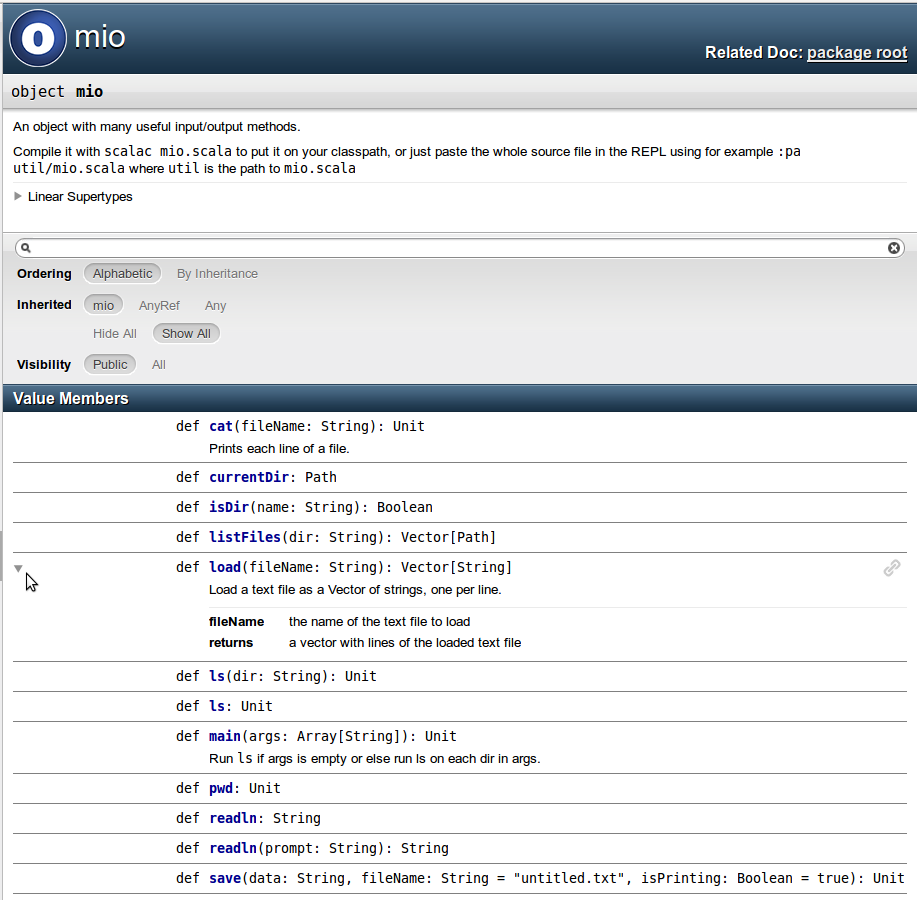
\includegraphics[width=1.0\textwidth]{../img/scaladoc/scaladoc-mio}
    \caption{Delar av en webbsida genererad med hjälp av \scaladoc. Mer detaljerade beskrivningar kan i förekommande fall vecklas ut eller in om man växlar mellan \Forward~och \MoveDown.}
    \label{fig:scaladoc:webpage}
\end{figure}


\subsection{Lära mer om scaladoc}

\begin{itemize}[leftmargin=*]

\item En video med tips om hur du söker och navigerar i \scaladoc-dokumentation: 
\\
\url{http://docs.scala-lang.org/overviews/scaladoc/interface.html}

\item
Riktlinjer för hur du skriver dokumentationskommentarer: \\
\url{http://docs.scala-lang.org/style/scaladoc.html}

\item Länksida till mer detaljerade beskrivningar: \\
\url{https://wiki.scala-lang.org/display/SW/Writing+Documentation} \\
inkluderande bland annat:

\begin{itemize}[nolistsep]
\item En beskrivning av syntaxen för formatering: \\
\url{https://wiki.scala-lang.org/display/SW/Syntax} 

\item En beskrivning av speciella annoteringar, t.ex. \code{@param}: \\
\url{https://wiki.scala-lang.org/display/SW/Tags+and+Annotations} 

\end{itemize}

\item Kör kommandot \texttt{ scaladoc -help } för att se användbara optioner.

\item \texttt{sbt doc} är ett smidigt sätt att generera api-dokumentation. Läs mer om \texttt{sbt} och api-dokumentation här: \\
\url{http://www.scala-sbt.org/0.13/docs/Howto-Scaladoc.html}


\end{itemize}

\clearpage

\section{javadoc}
\newcommand{\javadoc}{\texttt{javadoc}}


Med Java JDK följer dokumentationsverktyget \javadoc, som utifrån dokumentationskommentarer i Java-kod genererar en webbsajt med navigationslänkar. Webbsidor genererade med \javadoc~erbjuder inte samma funktioner för sökning och filtrering som \scaladoc, men det fungerar bra hitta det man söker om navigationslänkarna används tillsammans med webbläsarens inbyggda sökfunktion (Ctrlf+F).

\subsection{Använda dokumentation genererad med javadoc}

I figur \ref{fig:javadoc:overview} visas exempel på \javadoc~för biblioteket \code{cslib}. Om du klickar på ett paket kan du navigera till en översikt av innehållet i paketet. Om du klickar på en klass får du en översikt av klassens medlemmar, så som visas i \ref{fig:javadoc:class}.  Om du t.ex. klickar på ett metodnamn får du se mer detaljerade kommentarer. 

Ramarna till vänster på webbsidorna innehåller länkar till paket och klasser. Om du klickar på länken \textit{All Classes} överst till vänster för du en lista med navigationslänkar till alla tillgängliga klasser.De gulmarkerade rubrikerna visar vilken vy som är aktiv och navigationslänkar skrivs med blå text.

\begin{figure}
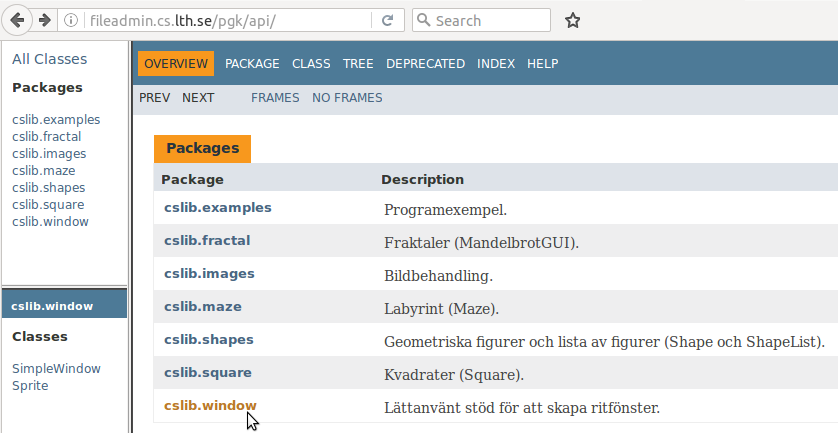
\includegraphics[width=1.0\textwidth]{../img/javadoc/javadoc-overview}
    \caption{Delar av en webbsida genererad med hjälp av \javadoc.}
    \label{fig:javadoc:overview}
\end{figure}



\begin{figure}
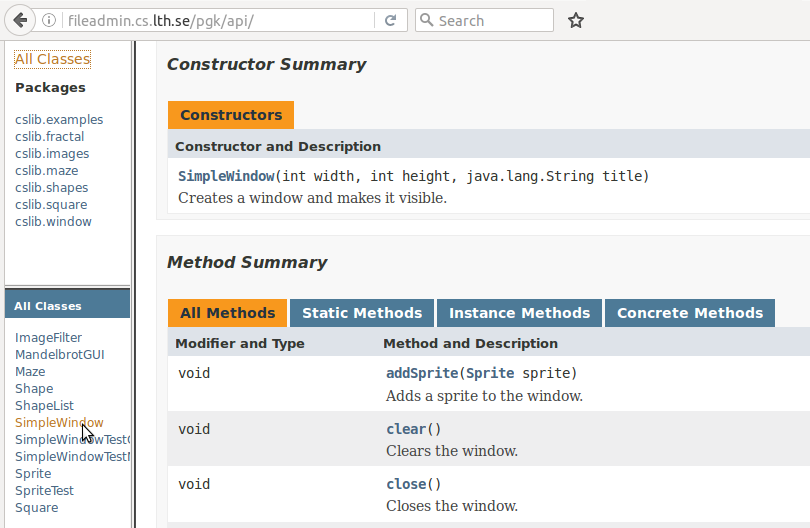
\includegraphics[width=1.0\textwidth]{../img/javadoc/javadoc-class}
    \caption{Delar av en webbsida med klassdokumentation genererad med hjälp av \javadoc.}
    \label{fig:javadoc:class}
\end{figure}






\subsection{Skriva dokumentationskommentarer för javadoc}

Kommentarer för \javadoc~och \scaladoc~ser ganska lika ut, även om det finns några skillnader. Det finns t.ex. inte lika många styrtecken för layouten i \javadoc~som i \scaladoc, och konventionen i Java är fyra blankstegs indrag och att fortsättningsrader i dokumentationskommentarer börjar asterisken under \textit{första} asterisken i öppningskommentaren. 

Nedan visas delar av \javadoc-kommentarerna för klassen \code{SimpleWindow} och dess konstruktor:
\begin{Code}[language=Java]
package cslib.window;
 
/** A simple window to draw in */
public class SimpleWindow {
   /**
    * Creates a window and makes it visible.
    * 
    * @param width   the width of the window
    * @param height  the height of the window
    * @param title   the title of the window
    */
    public SimpleWindow(int width, int height, String title) {
        ...
\end{Code}
Annoteringen \verb|@param| i början på en rad ger en speciell kommentar angående en parameter. Vid dokumentation av metoder kan annoteringen \verb|@return| användas i början av en rad för att skapa en speciell kommentar angående vad som returneras.

Övergripande dokumentation om innehållet i ett paket läggs i en textfil i paketets katalog med namnet \texttt{package-info.java}, se till exempel här: \\ {\href{https://github.com/lunduniversity/introprog/tree/master/workspace/cslib/src/main/java/cslib/window}{\small github.com/lunduniversity/introprog/tree/master/workspace/cslib/src/main/java/cslib/window}


Du kan läsa mer om hur man skriver \code{javadoc}-kommentarer här:\\
\href{http://www.oracle.com/technetwork/java/javase/documentation/index-137868.html}{www.oracle.com/technetwork/java/javase/documentation/index-137868.html}

% conversation of diffs between javadoc and scaladoc:
%  https://groups.google.com/forum/#!msg/scala-user/q-Vw03zcIVs/CaTR5XL-BQAJ

\subsection{Generera dokumentationskommentarer för javadoc}

Om du står i den katalog där din källkod finns, kan du med nedan kommando i terminalen gå igenom alla paket och underpaket och generera \javadoc-webbsidor i katalogen \texttt{doc}. Du kan därefter öppna dokumentationen i en webbläsare.
\begin{REPLnonum}[basicstyle=\color{white}\ttfamily\fontsize{9}{11}\selectfont]
$ javadoc -d doc -encoding UTF-8 -charset UTF-8 -sourcepath . -subpackages . *
$ firefox doc/index.html
\end{REPLnonum}
Ett smidigt sätt att generera både \scaladoc~och \javadoc~ är att använda \texttt{sbt}; det är bara att skriva \code{ sbt doc } i terminalen så genereras alla dokumentation för både Scala och Java i den katalog som \texttt{sbt} meddelar i sin resultatutskrift.

Om du lägger in nedan i \code{settings} i din \code{build.sbt} fungerar även svenska bokstäver och andra specialtecken på alla plattformar.
\begin{Code}
  javacOptions in (Compile, doc) ++= Seq(
    "-encoding", "UTF-8", 
    "-charset", "UTF-8", 
    "-docencoding", "UTF-8")
\end{Code}  

\noindent Du kan också använda din IDE för att köra \javadoc. I Eclipse, använd menyn \MenuArrow{Project}\Menu{Generate Javadoc...}, medan du i IntelliJ hittar motsvarande i menyn \MenuArrow{Tools}\Menu{Generate Javadoc...}